
        \documentclass[spanish, 11pt]{exam}

        %These tell TeX which packages to use.
        \usepackage{array,epsfig}
        \usepackage{amsmath, textcomp}
        \usepackage{amsfonts}
        \usepackage{amssymb}
        \usepackage{amsxtra}
        \usepackage{amsthm}
        \usepackage{mathrsfs}
        \usepackage{color}
        \usepackage{multicol, xparse}
        \usepackage{verbatim}


        \usepackage[utf8]{inputenc}
        \usepackage[spanish]{babel}
        \usepackage{eurosym}

        \usepackage{graphicx}
        \graphicspath{{../img/}}
        \usepackage{pgf}



        \printanswers
        \nopointsinmargin
        \pointformat{}

        %Pagination stuff.
        %\setlength{\topmargin}{-.3 in}
        %\setlength{\oddsidemargin}{0in}
        %\setlength{\evensidemargin}{0in}
        %\setlength{\textheight}{9.in}
        %\setlength{\textwidth}{6.5in}
        %\pagestyle{empty}

        \let\multicolmulticols\multicols
        \let\endmulticolmulticols\endmulticols
        \RenewDocumentEnvironment{multicols}{mO{}}
         {%
          \ifnum#1=1
            #2%
          \else % More than 1 column
            \multicolmulticols{#1}[#2]
          \fi
         }
         {%
          \ifnum#1=1
          \else % More than 1 column
            \endmulticolmulticols
          \fi
         }
        \renewcommand{\solutiontitle}{\noindent\textbf{Sol:}\enspace}

        \newcommand{\samedir}{\mathbin{\!/\mkern-5mu/\!}}

        \newcommand{\class}{1º Bachillerato}
        \newcommand{\examdate}{\today}

        \newcommand{\tipo}{A}


        \newcommand{\timelimit}{50 minutos}



        \pagestyle{head}
        \firstpageheader{
\includegraphics[width=0.2\columnwidth]{header_left}}{\textbf{Departamento de Matemáticas\linebreak \class}\linebreak \examnum}{
\includegraphics[width=0.1\columnwidth]{header_right}}
        \runningheader{\class}{\examnum}{Página \thepage\ of \numpages}
        \runningheadrule

        \newcommand{\examnum}{Ejercicios 13/05}
        \begin{document}
        \begin{questions}
        \question e1-0 - Halla analíticamente el dominio de las siguientes funciones y comprueba el resultado con la gráfica que aparece en la solución:
        \begin{multicols}{2}
        \begin{parts} \part[1] $f(x)=0x+3$  \begin{solution}   $Dom\left(f \right)=\mathbb{R}$\\ \resizebox{0.4\textwidth}{!}{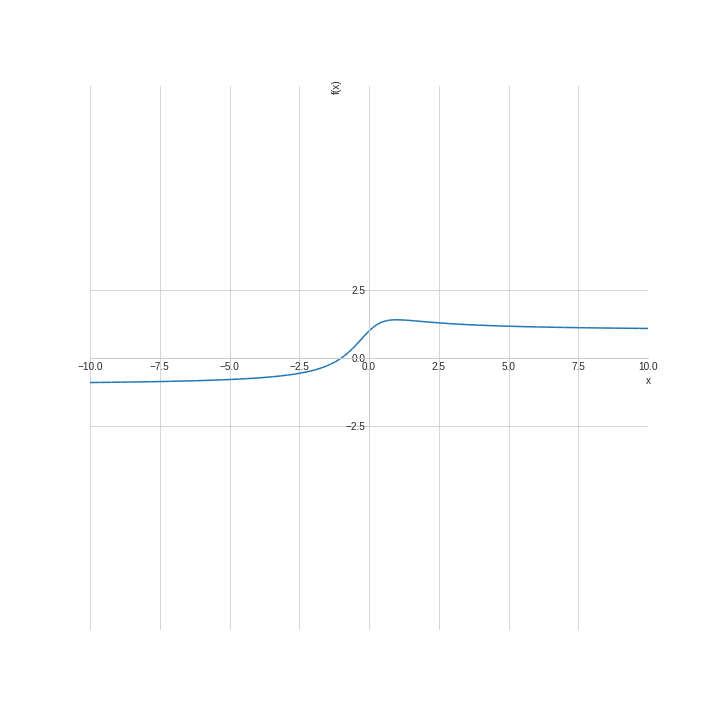
\includegraphics[width=1\columnwidth]{e1-0-0}}   \end{solution} \part[1] $f(x)=x^3-5x^2+2$  \begin{solution}   $Dom\left(f \right)=\mathbb{R}$\\ \resizebox{0.4\textwidth}{!}{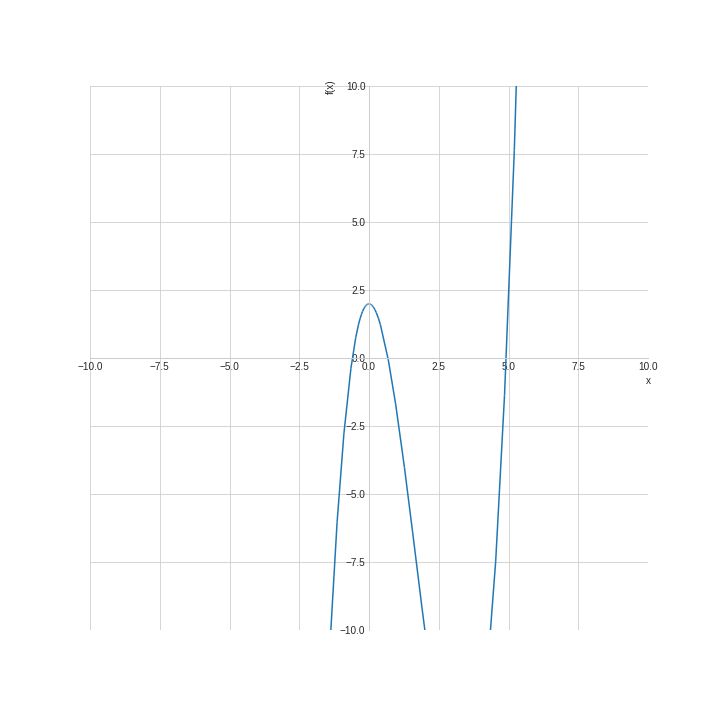
\includegraphics[width=1\columnwidth]{e1-0-1}}   \end{solution} \part[1] $f(x)=\frac{{x - 3}}{{x + 2}}$  \begin{solution}   $Dom\left(f \right)=\left(-\infty, -2\right) \cup \left(-2, \infty\right)$\\ \resizebox{0.4\textwidth}{!}{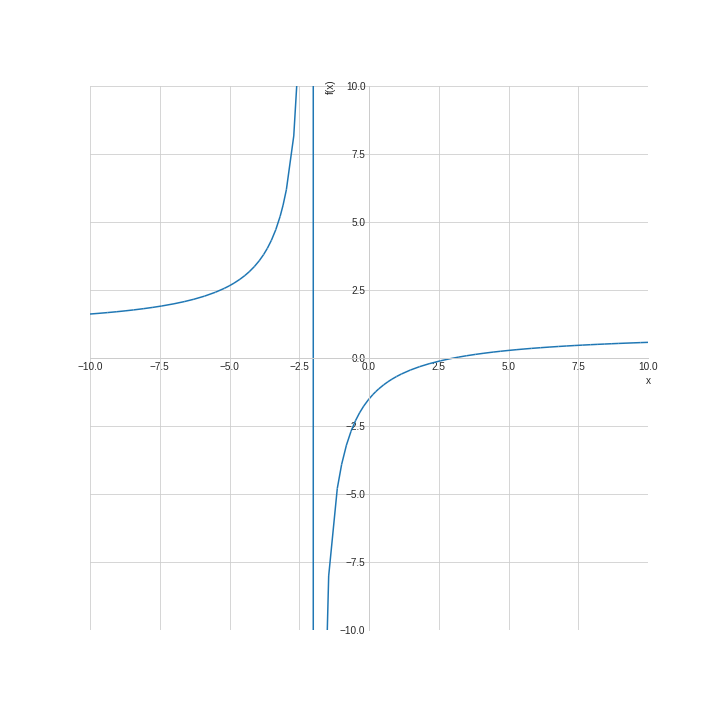
\includegraphics[width=1\columnwidth]{e1-0-2}}   \end{solution} \part[1] $f(x)=2x-3$  \begin{solution}   $Dom\left(f \right)=\mathbb{R}$\\ \resizebox{0.4\textwidth}{!}{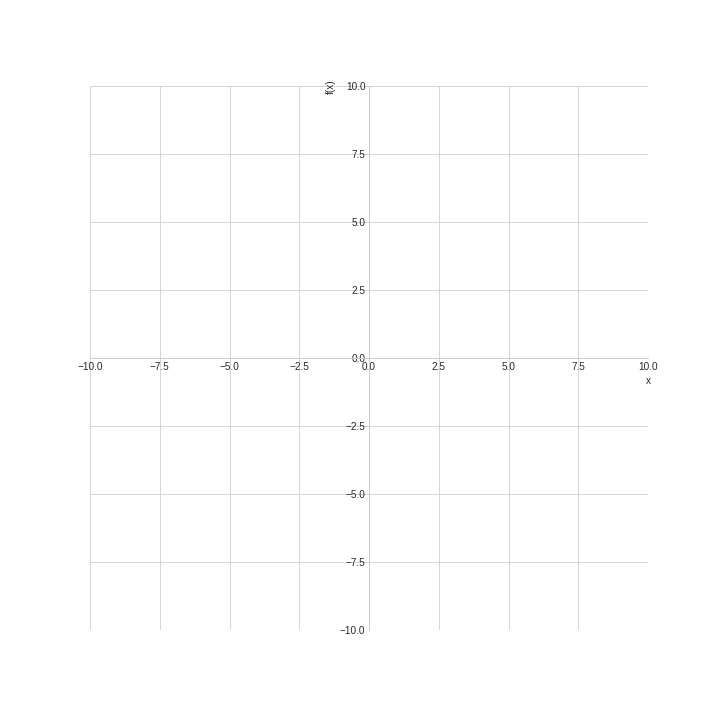
\includegraphics[width=1\columnwidth]{e1-0-3}}   \end{solution} \part[1] $f(x)=2-\frac{2}{x-1}$  \begin{solution}   $Dom\left(f \right)=\left(-\infty, 1\right) \cup \left(1, \infty\right)$\\ \resizebox{0.4\textwidth}{!}{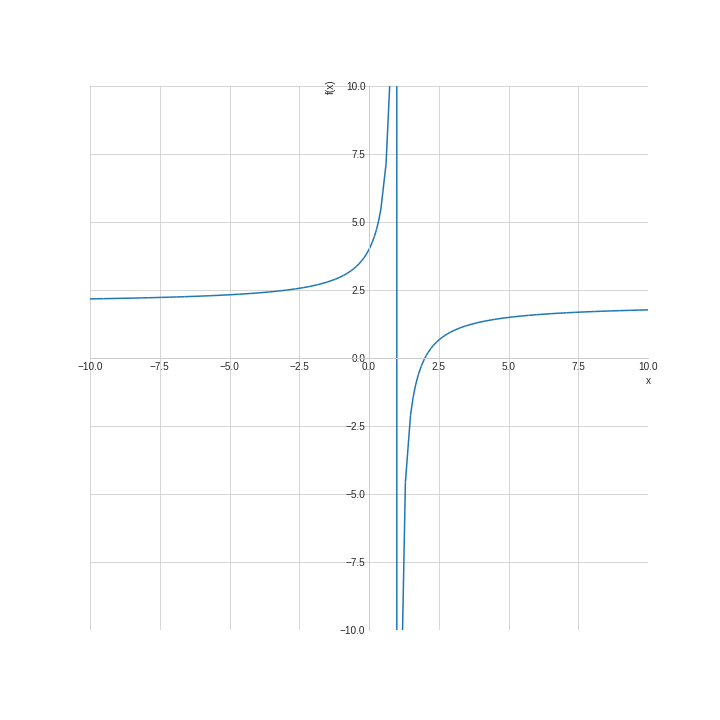
\includegraphics[width=1\columnwidth]{e1-0-4}}   \end{solution}
        \end{parts}
        \end{multicols}
        \question e1b-0 - Halla analíticamente el dominio de las siguientes funciones:
        \begin{multicols}{3}
        \begin{parts} \part[1] $f(x)=\sqrt[3]{\frac{x + 2}{x - 3}}$  \begin{solution}   $Dom\left(f \right)=\left(-\infty, 3\right) \cup \left(3, \infty\right)$   \end{solution} \part[1] $f(x)=\sqrt {\frac{x}{2 x^{2} + 2 x - 12}}$  \begin{solution}   $Dom\left(f \right)=\left(-\infty, -3\right) \cup \left(2, \infty\right)$   \end{solution} \part[1] $f(x)=\sqrt {x^2-9}$  \begin{solution}   $Dom\left(f \right)=\left(-\infty, -3\right] \cup \left[3, \infty\right)$   \end{solution}
        \end{parts}
        \end{multicols}
        \question e3-0 - Dadas las funciones $f(x)= x^2+4$, $g(x)= \frac{{x - 1}}{{x + 2}}$ y $h(x)= \sqrt{2x}$. Calcula: 
    
        \begin{multicols}{3}
        \begin{parts} \part[1] $g \circ f$  \begin{solution}   $g{\left(f{\left(x \right)} \right)}=\frac{x^{2} + 3}{x^{2} + 6}$   \end{solution} \part[1] $f \circ g$  \begin{solution}   $f{\left(g{\left(x \right)} \right)}=\frac{\left(x - 1\right)^{2}}{\left(x + 2\right)^{2}} + 4$   \end{solution} \part[1] $h \circ g \circ f$  \begin{solution}   $h{\left(g{\left(f{\left(x \right)} \right)} \right)}=\frac{\sqrt{2} \sqrt{x^{2} + 3}}{\sqrt{x^{2} + 6}}$   \end{solution}
        \end{parts}
        \end{multicols}
        \question e4 - Halla la función inversa de $f(x)$, y comprueba el resultado, siendo:
        \begin{multicols}{2}
        \begin{parts} \part[1] $f(x)=5 x - 1$  \begin{solution}   $f^{-1}(x)=\frac{x}{5} + \frac{1}{5}$ \\ $f^{-1} \circ f(x)=x=x$ \\\\ \resizebox{0.4\textwidth}{!}{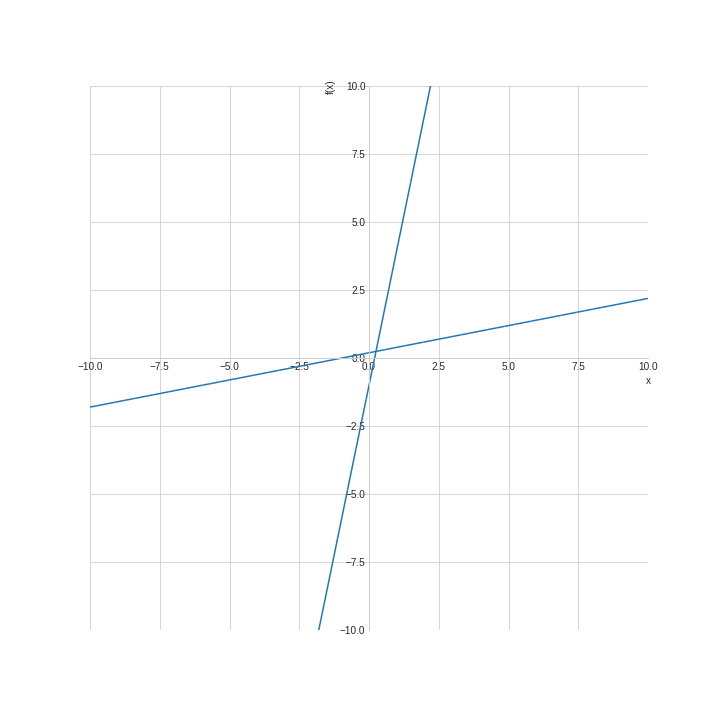
\includegraphics[width=1\columnwidth]{e4-0}}   \end{solution} \part[1] $f(x)=\frac{x + 1}{2 - x}$  \begin{solution}   $f^{-1}(x)=\frac{2 x - 1}{x + 1}$ \\ $f^{-1} \circ f(x)=\frac{-1 + \frac{2 \left(x + 1\right)}{2 - x}}{1 + \frac{x + 1}{2 - x}}=x$ \\\\ \resizebox{0.4\textwidth}{!}{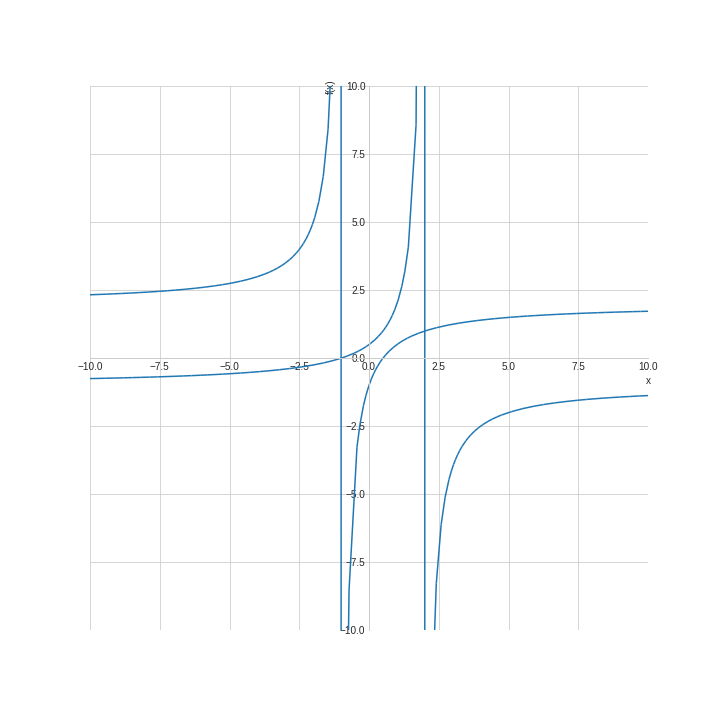
\includegraphics[width=1\columnwidth]{e4-1}}   \end{solution}
        \end{parts}
        \end{multicols}
        \question e5 - Calcula los siguientes límites:

        \begin{multicols}{3}
        \begin{parts} \part[1] $\lim_{x \to 3}\left(\left(x^{2} - 3 x\right) - 1\right)$  \begin{solution}   $-1$   \end{solution} \part[1] $\lim_{x \to 2}\left(\frac{\left(x^{2} - 10 x\right) + 4}{x}\right)$  \begin{solution}   $-6$   \end{solution} \part[1] $\lim_{x \to 4}\left(\frac{2 x - 1}{\sqrt{x}}\right)$  \begin{solution}   $\frac{7}{2}$   \end{solution} \part[1] $\lim_{x \to 3}\left(\frac{1 - x}{\left(3 - x\right)^{2}}\right)$  \begin{solution}   $-\infty$   \end{solution} \part[1] $\lim_{x \to 3}\left(\frac{7}{\left(x^{2} - 6 x\right) + 9}\right)$  \begin{solution}   $\infty$   \end{solution} \part[1] $\lim_{x \to 0}\left(\frac{x - 1}{x^{2}}\right)$  \begin{solution}   $-\infty$   \end{solution} \part[1] $\lim_{x \to 2}\left(\frac{\left(x^{2} - x\right) - 2}{\left(3 x^{2} + 12 x\right) + 12}\right)$  \begin{solution}   $0$   \end{solution} \part[1] $\lim_{x \to 1}\left(\frac{x - 1}{\sqrt{x} - 1}\right)$  \begin{solution}   $2$   \end{solution}
        \end{parts}
        \end{multicols}
        
    \end{questions}
    \end{document}
    